\documentclass[letterpaper,10pt]{book}
% Change to 10 pt
\usepackage{pdfpages}
\usepackage{morewrites}			% to counteract the no write space problem
\setcounter{tocdepth}{6}

\usepackage[framemethod=TikZ]{mdframed}

\usepackage{fancyhdr}

\usepackage{paralist}
\usepackage{amsmath}
\usepackage{amsfonts}
\usepackage{amssymb}
\usepackage{graphicx}

\usepackage{datetime}
%\usepackage{ulem}

%\usepackage[nottoc]{toobibind}

\usepackage[inline]{enumitem}

% Outer margin at 2.50 is exacty correct to fit the ``corruption alert'' tables
\usepackage[inner=1.0in, outer=2.50in, top=2.54cm,bottom=2.54cm, marginparwidth=2.25in]{geometry}

\usepackage{marginnote}
\usepackage{longtable}
\usepackage{booktabs}
\usepackage{xcolor}

\usepackage{soul}

%%%%%%%%%%%%
\definecolor{ForestGreen}{rgb}{0.00,0.29,0.098}
%%%%%%%%%%%%

\usepackage{marginnote}

\usepackage{imakeidx} 
\usepackage[
	backref=true,
	style=numeric,
%	citestyle=numeric,
	backend=bibtex
	]{biblatex}
\usepackage[driverfallback=hypertex,colorlinks=True]{hyperref}
\usepackage{cleveref}

\makeindex[name=scripture,columnsep=20pt, columnseprule=True,columns=3, title=Scripture References]
\makeindex[name=speaker,columnsep=20pt, columnseprule=True,,columns=2, title=Sermon Creator]
\makeindex[name=series,columnsep=20pt, columnseprule=True,,columns=2, title=Sermon Series]
\makeindex[name=date,columnsep=20pt, columnseprule=True,columns=2, title=Sermon Date]
\makeindex[name=event,columnsep=20pt, columnseprule=True,columns=2, title=Event]
\makeindex[name=topic,columnsep=20pt, columnseprule=True,columns=2, title=Topic]
\makeindex[name=AWIP,columnsep=20pt, columnseprule=True,columns=3, title=All Words in Passage]
\makeindex[name=NWIV,columnsep=20pt, columnseprule=True,columns=3, title=Number of Words in Verse]
\makeindex[name=PNIP,columnsep=20pt, columnseprule=True,columns=3, title=Proper Names in Passage]
\makeindex[name=PEIP,columnsep=20pt, columnseprule=True,columns=2, title=Prophetic Events in Passage]
\makeindex[name=TWPAQ,columnsep=20pt, columnseprule=True,columns=1, title=13-Word Phrases and Quotes]
\makeindex[name=PFTTIS,columnsep=20pt, columnseprule=False,columns=3, title=Phrases found 13 times in scripture]
\makeindex[name=WFTTIS,columnsep=20pt, columnseprule=False,columns=3, title=Words found 13 times in scripture]
\makeindex[name=WFITV,columnsep=20pt, columnseprule=False,columns=3, title=Words found in exactly 13 verses]
\makeindex[name=EVENTS,columnsep=20pt, columnseprule=False,columns=2, title=Sermon Log by Place]
\makeindex[name=QUESTIONS,columnsep=20pt, columnseprule=False,columns=2, title=Bible Questions]
\makeindex[name=DOCTRINES,columnsep=20pt, columnseprule=False,columns=2, title=Doctrines]
\makeindex[name=SONGS,columnsep=20pt, columnseprule=False,columns=1, title=Songs]
\makeindex[name=LOCATION,columnsep=20pt, columnseprule=False,columns= 2, title=Location]
\makeindex[name=FACEBOOK,columnsep=20pt, columnseprule=False,columns=2, title=Facebook]
\makeindex[name=DEVOTIONAL,columnsep=20pt, columnseprule=False,columns=2, title=Devotional Items]
%%%%%%%%%%%%%%%%% EXTRA COLORS
\definecolor{champagne}{rgb}{0.97,0.91,0.81}
\definecolor{bone}{rgb}{0.89,0.85,0.79}
\pagestyle{fancy}
\fancyhf{}
\fancyhead[LE,RO]{\today}
\fancyhead[RE,LO]{Daily Bible Reading}
\fancyhead[CE,CO]{-page \thepage  - }

\fancyfoot[CO,CE]{\leftmark}
%\fancyfoot[LE,RO]{CSCE 692, HW1}

\title{DBR\\
Daily \\ Reads}
\author{Keith Anthony \\
\today }
%+/ffffff +   \pagenumbering{gobble}
\bibliography{Bibliographies/All20220122}

\setlength{\fboxsep}{1.0pt}

\usepackage[utf8]{inputenc}
\usepackage{tikz}

\begin{document}
%%%%%%%%%%%% Tile Page

\begin{titlepage}

\begin{flushright}
\rightskip=-2.5cm
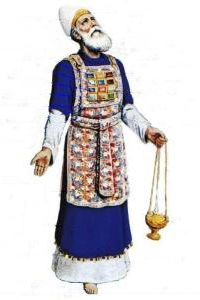
\includegraphics[width=50mm,scale=1.5]{Extras/Melchisedec.jpg}
\vspace{0.4in}  % Create a title for the document and write it in bold font
\LARGE{\textbf{\date}} % Again, do a line break
\linebreak 
% Create a subtitle \large{with Outlines, Statistics, Cross References, and Notes}
\vspace{0.5in}
\begin{flushleft}
\LARGE{Day \#47: Wednesday, 16 February 2022 PLAIN  \\}\vspace{0.25in}
\LARGE{Numbers 19-21 Psalm 47 Proverb 16}
\end{flushleft}
\vspace{0.6in}
\bigskip

\normalsize{Xenia, Oh.\\}
\normalsize{created: \today}
\vspace{1.3in}

\end{flushright}
\end{titlepage}

\newpage 
\tableofcontents\hypertarget{TOC}{}

\hyphenation{A-bim-e-lech bre-thren E-phra-im  Gib-e-o-nites Jer-u-sa-lem through-out Phil-i-stines The-o-phil-us Am-a-le-kites ven-geance Mesh-el-e-mi-ah onan-ism Phar-a-oh thoughts grev-ous-ness Hach-a-liah adul-ter-er Shad-rach}

%%%%%%%%%%%%%%%%% EXTRA COLORS
%%%%%%%%%%%%%%%%% EXTRA COLORS
%%%%%%%%%%%%%%%%% EXTRA COLORS
\definecolor{champagne}{rgb}{0.97,0.91,0.81}
\definecolor{bone}{rgb}{0.89,0.85,0.79}

\definecolor{ForestGreen}{rgb}{0.00,0.29,0.098}
\definecolor{GIVING}{cmyk}{1,0.0,0.72,.1}

\definecolor{MLPE}{cmyk}{1,1,0,.45}
\definecolor{SOCCER}{cmyk}{.77, 0, .42, .49}
\definecolor{PAYBILL}{cmyk}{0,0.83,0.76,0.07}
\definecolor{SERMON}{cmyk}{.14,.9,0,.30} % aka seance \href{http://www.flatuicolorpicker.com/purple-cmyk-color-model/}{seance}
\definecolor{BIBLE}{cmyk}{0,.17,.74,.17}
\definecolor{WORKBLUE}{cmyk}{1, .5, 0, .6}
\definecolor{myOrange}{cmyk}{0, .4, .98, .03}
\definecolor{myTan}{cmyk}{0.0,.07,.17,.10}
\definecolor{myRed}{cmyk}{0,1,1,0}
\definecolor{myWhite}{cmyk}{0,0,0,0}
\definecolor{BLUESoD}{cmyk}{.97,.84,0,.04}
\definecolor{WHITE}{cmyk}{0,0,0,0}
\definecolor{OLDGOLD}{cmyk}{0.05,0.3,1.00,0}
\definecolor{CASTLETON}{cmyk}{1,0,0.31,0.66}
\definecolor{cadmiumgreen}{rgb}{0.0, 0.42, 0.24}
\definecolor{jungle}{rgb}{0.203,0.4882,0.1718}
\definecolor{MYGOLD}{rgb}{1,.84,0}

\definecolor{MYLIGHTGRAY}{rgb}{.85,.85,.85}

\definecolor{codegreen}{rgb}{0,0.6,0}
\definecolor{codegray}{rgb}{0.5,0.5,0.5}
\definecolor{codepurple}{rgb}{0.58,0,0.82}
\definecolor{backcolour}{rgb}{0.95,0.95,0.92}


\mdfdefinestyle{MyFrame}{%
    linecolor=blue,
    outerlinewidth=2pt,
    roundcorner=5pt,
    innertopmargin=\baselineskip,
    innerbottommargin=\baselineskip,
    innerrightmargin=10pt,
    innerleftmargin=10pt,
    backgroundcolor=gray!25!white}


\mdfdefinestyle{MyFrame2}{%
    linecolor=black,
    outerlinewidth=2pt,
    roundcorner=5pt,
    innertopmargin=\baselineskip,
    innerbottommargin=\baselineskip,
    innerrightmargin=10pt,
    innerleftmargin=10pt,
    backgroundcolor=yellow!25!white}


%%%%%
%% for PFTTIS list
%%%%%

%%% And Joseph said unto
\index[PFTTIS]{And Joseph said unto!Genesis!Gen 40:008}
\index[PFTTIS]{And Joseph said unto!Genesis!Gen 40:012}
\index[PFTTIS]{And Joseph said unto!Genesis!Gen 41:025}
\index[PFTTIS]{And Joseph said unto!Genesis!Gen 42:014}
\index[PFTTIS]{And Joseph said unto!Genesis!Gen 42:018}
\index[PFTTIS]{And Joseph said unto!Genesis!Gen 44:015}
\index[PFTTIS]{And Joseph said unto!Genesis!Gen 45:003}
\index[PFTTIS]{And Joseph said unto!Genesis!Gen 45:004}
\index[PFTTIS]{And Joseph said unto!Genesis!Gen 46:031}
\index[PFTTIS]{And Joseph said unto!Genesis!Gen 48:009}
\index[PFTTIS]{And Joseph said unto!Genesis!Gen 48:018}
\index[PFTTIS]{And Joseph said unto!Genesis!Gen 50:019}
\index[PFTTIS]{And Joseph said unto!Genesis!Gen 50:024}


%%% a shadow
\index[PFTTIS]{a shadow!1Chronicles!1Chr 029:15}
\index[PFTTIS]{a shadow!Job!Job 008:09}
\index[PFTTIS]{a shadow!Job!Job 014:02}
\index[PFTTIS]{a shadow!Job!Job 017:07}
\index[PFTTIS]{a shadow!Psalm!Psa 102:011}
\index[PFTTIS]{a shadow!Psalm!Psa 144:004}
\index[PFTTIS]{a shadow!Ecclesiastes!Eccl 006:012}
\index[PFTTIS]{a shadow!Ecclesiastes!Eccl 008:013}
\index[PFTTIS]{a shadow!Isaiah!Isa 04:006}
\index[PFTTIS]{a shadow!Isaiah!Isa 25:004}
\index[PFTTIS]{a shadow!Jonah!Jnh 04:06}
\index[PFTTIS]{a shadow!Colossians!Col 02:017}
\index[PFTTIS]{a shadow!Hebews!Heb 10:001}

%%% blessed is the man
\index[PFTTIS]{blessed is the man!Psalm!Psa 001:001}
\index[PFTTIS]{blessed is the man!Psalm!Psa 032:002}
\index[PFTTIS]{blessed is the man!Psalm!Psa 034:008}
\index[PFTTIS]{blessed is the man!Psalm!Psa 065:004}
\index[PFTTIS]{blessed is the man!Psalm!Psa 084:005}
\index[PFTTIS]{blessed is the man!Psalm!Psa 084:012}
\index[PFTTIS]{blessed is the man!Psalm!Psa 094:012}
\index[PFTTIS]{blessed is the man!Psalm!Psa 112:001}
\index[PFTTIS]{blessed is the man!Proverbs!Pro 008:034}
\index[PFTTIS]{blessed is the man!Isaiah!Isa 056:002}
\index[PFTTIS]{blessed is the man!Jeremiah!Jer 017:007}
\index[PFTTIS]{blessed is the man!Romans!Rom 004:008}
\index[PFTTIS]{blessed is the man!James!Jam 001:012}


%%% carry them
\index[PFTTIS]{carry them!Leviticus!Lev 14:045}
\index[PFTTIS]{carry them!Numbers!Num 11:012}
\index[PFTTIS]{carry them!Joshua!Jsh 04:003}
\index[PFTTIS]{carry them!1Samuel!1Sam 20:040}
\index[PFTTIS]{carry them!1Kings!1Kng 08:046}
\index[PFTTIS]{carry them!2Chronicles!2Chr 06:036}
\index[PFTTIS]{carry them!Ezra!Ezra 05:015}
\index[PFTTIS]{carry them!Isaiah!Isa 40:011}
\index[PFTTIS]{carry them!Isaiah!Isa 41:016}
\index[PFTTIS]{carry them!Isaiah!Isa 57:013}
\index[PFTTIS]{carry them!Jeremiah!Jer 20:004}
\index[PFTTIS]{carry them!Jeremiah!Jer 20:005}
\index[PFTTIS]{carry them!Jeremiah!Jer 43:012}


\index[PFTTIS]{good tidings!2Samuel!2Sam 18:027}
\index[PFTTIS]{good tidings!1Kings!1Ki 01:042}
\index[PFTTIS]{good tidings!2Kings!2Ki 07:009 (2x)}
\index[PFTTIS]{good tidings!Isaiah!Isa 40:009 (2x)}
\index[PFTTIS]{good tidings!Isaiah!Isa 41:007}
\index[PFTTIS]{good tidings!Isaiah!Isa 52:007}
\index[PFTTIS]{good tidings!Isaiah!Isa 61:001}
\index[PFTTIS]{good tidings!Nahum!Nah 01:005}
\index[PFTTIS]{good tidings!Luke!Lk 02:010}
\index[PFTTIS]{good tidings!1Thessalonians!1Thess 03:006}


%%% dead body
\index[PFTTIS]{dead body!Leviticus!Lev 21:011}
\index[PFTTIS]{dead body!Numbers!Num 06:006}
\index[PFTTIS]{dead body!Numbers!Num 09:006}
\index[PFTTIS]{dead body!Numbers!Num 09:007}
\index[PFTTIS]{dead body!Numbers!Num 09:010}
\index[PFTTIS]{dead body!Numbers!Num 09:011}
\index[PFTTIS]{dead body!Numbers!Num 09:013}
\index[PFTTIS]{dead body!Numbers!Num 09:016}
\index[PFTTIS]{dead body!2Kings!2Ki 08:005}
\index[PFTTIS]{dead body!Isaiah!Isa 26:019}
\index[PFTTIS]{dead body!Jeremiah!Jer 26:023}
\index[PFTTIS]{dead body!Jeremiah!Jer 36:030}
\index[PFTTIS]{dead body!Haggai!Hag 02:013}

%%% great sea
\index[PFTTIS]{great sea!Numbers!Num 34:006}
\index[PFTTIS]{great sea!Numbers!Num 34:007}
\index[PFTTIS]{great sea!Joshua!Jos 01:004}
\index[PFTTIS]{great sea!Joshua!Jos 09:001}
\index[PFTTIS]{great sea!Joshua!Jos 15:012}
\index[PFTTIS]{great sea!Joshua!Jos 15:047}
\index[PFTTIS]{great sea!Joshua!Jos 23:004}
\index[PFTTIS]{great sea!Ezekiel!Eze 47:010}
\index[PFTTIS]{great sea!Ezekiel!Eze 47:015}
\index[PFTTIS]{great sea!Ezekiel!Eze 47:019}
\index[PFTTIS]{great sea!Ezekiel!Eze 47:020}
\index[PFTTIS]{great sea!Ezekiel!Eze 48:028}
\index[PFTTIS]{great sea!Daniel!Dan 07:002}


%%% have forsaken me
\index[PFTTIS]{have forsaken me!Judges!Jdg 10:013}
\index[PFTTIS]{have forsaken me!1Samuel!1Sam 08:008}
\index[PFTTIS]{have forsaken me!1Kings!1Ki 11:033}
\index[PFTTIS]{have forsaken me!2Kings!2Ki 22:017}
\index[PFTTIS]{have forsaken me!2Chronicles!2Chr 12:005}
\index[PFTTIS]{have forsaken me!2Chronicles!2Chr 34:025}
\index[PFTTIS]{have forsaken me!Jeremiah!Jer 01:016}
\index[PFTTIS]{have forsaken me!Jeremiah!Jer 02:013}
\index[PFTTIS]{have forsaken me!Jeremiah!Jer 05:007}
\index[PFTTIS]{have forsaken me!Jeremiah!Jer 05:019}
\index[PFTTIS]{have forsaken me!Jeremiah!Jer 16:011 (2x)}
\index[PFTTIS]{have forsaken me!Jeremiah!Jer 19:004}

%%% no king
\index[PFTTIS]{no king!Judges!Jdg 17:06}
\index[PFTTIS]{no king!Judges!Jdg 18:01}
\index[PFTTIS]{no king!Judges!Jdg 19:01}
\index[PFTTIS]{no king!Judges!Jdg 21:25}
\index[PFTTIS]{no king!1Kings!1Ki 22:47}
\index[PFTTIS]{no king!2Kings!2Ki 23:25}
\index[PFTTIS]{no king!Nehemiah!Neh 13:26}
\index[PFTTIS]{no king!Psalms!Psa 033:016}
\index[PFTTIS]{no king!Proverbs!Pro 30:27}
\index[PFTTIS]{no king!Daniel!Dan 02:10}
\index[PFTTIS]{no king!Hosea!Hos 10:03}
\index[PFTTIS]{no king!Micah!Mic 04:09}
\index[PFTTIS]{no king!John!Jhn 19:15}


%%% rebellious house
\index[PFTTIS]{rebellious house!Exodus!Exo 02:005}
\index[PFTTIS]{rebellious house!Exodus!Exo 02:006}
\index[PFTTIS]{rebellious house!Exodus!Exo 02:008}
\index[PFTTIS]{rebellious house!Exodus!Exo 03:009}
\index[PFTTIS]{rebellious house!Exodus!Exo 03:026}
\index[PFTTIS]{rebellious house!Exodus!Exo 03:027}
\index[PFTTIS]{rebellious house!Exodus!Exo 12:002 (2x)}
\index[PFTTIS]{rebellious house!Exodus!Exo 12:003}
\index[PFTTIS]{rebellious house!Exodus!Exo 12:009}
\index[PFTTIS]{rebellious house!Exodus!Exo 12:025}
\index[PFTTIS]{rebellious house!Exodus!Exo 17:012}
\index[PFTTIS]{rebellious house!Exodus!Exo 24:003}

%%% seek him
\index[PFTTIS]{seek him!Deuteronomy!Deu 04:029}\index[PFTTIS]{seek him!1Samuel!1Sam 23:025}
\index[PFTTIS]{seek him!1Chronicles!1Chr 28:009}
\index[PFTTIS]{seek him!2Chronicles!1Chr 15:002}
\index[PFTTIS]{seek him!Ezra!Ezr 08:022}
\index[PFTTIS]{seek him!Psalms!Psa 022:026}
\index[PFTTIS]{seek him!Psalms!Psa 024:006}
\index[PFTTIS]{seek him!Psalms!Psa 119:002}
\index[PFTTIS]{seek him!SoS!SoS 03:002}
\index[PFTTIS]{seek him!SoS!SoS 06:001}
\index[PFTTIS]{seek him!Hosea!Hos 07:010}
\index[PFTTIS]{seek him!Amos!Amo 05:008}
\index[PFTTIS]{seek him!Hebrews!Heb 11:0063}


%%% seek ye
\index[PFTTIS]{seek ye!Isaiah!Isa 34:016}
\index[PFTTIS]{seek ye!Isaiah!Isa 45:019}
\index[PFTTIS]{seek ye!Isaiah!Isa 55:006}
\index[PFTTIS]{seek ye!Amos!Amos 5:004}
\index[PFTTIS]{seek ye!John!John 1:38}
\index[PFTTIS]{seek ye!John!John 18:4}
\index[PFTTIS]{seek ye!John!John 18:7}
\index[PFTTIS]{seek ye!Matthew!Matt 6:33}
\index[PFTTIS]{seek ye!Numbers!Num 16:10}
\index[PFTTIS]{seek ye!Luke!Luke 12:31}
\index[PFTTIS]{seek ye!Luke!Luke 24:5}
\index[PFTTIS]{seek ye!Psalm!Psa 27:8}
\index[PFTTIS]{seek ye!Zephaniah!Zeph 2:3}

%%% the uncircumcised
\index[PFTTIS]{the uncircumcised!Genesis!Gen 17:014}
\index[PFTTIS]{the uncircumcised!Judges!Jdg 14:003}
\index[PFTTIS]{the uncircumcised!Judges!Jdg 15:018}
\index[PFTTIS]{the uncircumcised!2Samuel!2Sam 01:020}
\index[PFTTIS]{the uncircumcised!Isaiah!Isa 02:001}
\index[PFTTIS]{the uncircumcised!Jeremiah!Jer 09:025}
\index[PFTTIS]{the uncircumcised!Ezekiel!Eze 28:010}
\index[PFTTIS]{the uncircumcised!Ezekiel!Eze 31:018}
\index[PFTTIS]{the uncircumcised!Ezekiel!Eze 32:019}
\index[PFTTIS]{the uncircumcised!Ezekiel!Eze 32:027}
\index[PFTTIS]{the uncircumcised!Ezekiel!Eze 32:028}
\index[PFTTIS]{the uncircumcised!Ezekiel!Eze 32:029}
\index[PFTTIS]{the uncircumcised!Ezekiel!Eze 32:032}

%%% worship him
\index[PFTTIS]{worship him!Psalms!Psa 97:007}
\index[PFTTIS]{worship him!Zephaniah!Zeph 02:011}
\index[PFTTIS]{worship him!Matthew!Matt 02:002}
\index[PFTTIS]{worship him!Matthew!Matt 02:008}
\index[PFTTIS]{worship him!John!John 04:023}
\index[PFTTIS]{worship him!John!John 04:024 (2x)} 
\index[PFTTIS]{worship him!Acts!Acts 17:023}
\index[PFTTIS]{worship him!Hebrews!Heb 01:006}
\index[PFTTIS]{worship him!Revelation!Rev 04:010}
\index[PFTTIS]{worship him!Revelation!Rev 13:008}
\index[PFTTIS]{worship him!Revelation!Rev 14:007}
\index[PFTTIS]{worship him!Revelation!Rev 19:010}


%%%%%
%% for PFTTIS list
%%%%%

%%% afflictions
\index[WFTTIS]{afflictions!Psalms!Psa 34:019}
\index[WFTTIS]{afflictions!Psalms!Psa 132:001}
\index[WFTTIS]{afflictions!Acts!Acts 07:010}
\index[WFTTIS]{afflictions!Acts!Acts 20:023}
\index[WFTTIS]{afflictions!2Corinthians!2Cor 06:004}
\index[WFTTIS]{afflictions!Colossians!Col 01:024}
\index[WFTTIS]{afflictions!1Thessalonians!1Thess 03:003}
\index[WFTTIS]{afflictions!2Timothy!2Tim 01:008}
\index[WFTTIS]{afflictions!2Timothy!2Tim 03:011}
\index[WFTTIS]{afflictions!2Timothy!2Tim 04:005}
\index[WFTTIS]{afflictions!Hebrews!Heb 10:032}
\index[WFTTIS]{afflictions!Hebrews!Heb 10:033}
\index[WFTTIS]{afflictions!1Peter!1Pet 05:009}

%%% acsend
\index[WFTTIS]{acsend!Joshua!Jos 06:05}
\index[WFTTIS]{acsend!Psalm!Psa 024:003}
\index[WFTTIS]{acsend!Psalm!Psa 135:007}
\index[WFTTIS]{acsend!Psalm!Psa 139:008}
\index[WFTTIS]{acsend!Isaiah!Isa 14:013}
\index[WFTTIS]{acsend!Isaiah!Isa 14:014}
\index[WFTTIS]{acsend!Jeremiah!Jer 10:013}
\index[WFTTIS]{acsend!Jeremiah!Jer 51:016}
\index[WFTTIS]{acsend!Ezekiel!Eze 38:009}
\index[WFTTIS]{acsend!John!John 06:062}
\index[WFTTIS]{acsend!John!John 20:017}
\index[WFTTIS]{acsend!Romans!Rom 10:006}
\index[WFTTIS]{acsend!Revelation!Rev 17:008}

%%% Assyrian
\index[WFTTIS]{Assyrian!Isaiah!Isa 10:005}
\index[WFTTIS]{Assyrian!Isaiah!Isa 10:024}
\index[WFTTIS]{Assyrian!Isaiah!Isa 14:025}
\index[WFTTIS]{Assyrian!Isaiah!Isa 19:023}
\index[WFTTIS]{Assyrian!Isaiah!Isa 23:013}
\index[WFTTIS]{Assyrian!Isaiah!Isa 30:031}
\index[WFTTIS]{Assyrian!Isaiah!Isa 31:008}
\index[WFTTIS]{Assyrian!Isaiah!Isa 52:004}
\index[WFTTIS]{Assyrian!Ezekiel!Eze 31:003}
\index[WFTTIS]{Assyrian!Hosea!Hos 05:013}
\index[WFTTIS]{Assyrian!Hosea!Hos 11:005}
\index[WFTTIS]{Assyrian!Micah!Hos 05:005}
\index[WFTTIS]{Assyrian!Micah!Hos 05:006}

%%% blot
\index[WFTTIS]{blot!Exodus!Exo 32:032}
\index[WFTTIS]{blot!Exodus!Exo 32:033}
\index[WFTTIS]{blot!Numbers!Num 05:026}
\index[WFTTIS]{blot!Deuteronomy!Deut 09:014}
\index[WFTTIS]{blot!Deuteronomy!Deut 25:019}
\index[WFTTIS]{blot!Deuteronomy!Deut 29:020}
\index[WFTTIS]{blot!2Kings!2Ki 14:027}
\index[WFTTIS]{blot!Job!Job 31:007}
\index[WFTTIS]{blot!Psalms!Psa 51:001}
\index[WFTTIS]{blot!Psalms!Psa 51:009}
\index[WFTTIS]{blot!Proverbs!Pro 09:007}
\index[WFTTIS]{blot!Jeremiah!Jer 18:023}
\index[WFTTIS]{blot!Revelation!Rev 03:005}


%%% chain
\index[WFTTIS]{chain!Genesis!Gen 41:042}
\index[WFTTIS]{chain!1Kings!1Ki 07:017}
\index[WFTTIS]{chain!Psalms!Psa 73:006}
\index[WFTTIS]{chain!SoS!Sos 04:009}
\index[WFTTIS]{chain!Lamentations!Lam 03:007}
\index[WFTTIS]{chain!Ezekiel!Eze 07:023}
\index[WFTTIS]{chain!Ezekiel!Eze 16:011}
\index[WFTTIS]{chain!Daniel!Dan 05:007}
\index[WFTTIS]{chain!Daniel!Dan 05:016}
\index[WFTTIS]{chain!Daniel!Dan 05:029}
\index[WFTTIS]{chain!Acts!Acts 28:020}
\index[WFTTIS]{chain!2Timothy!2Tim 01:016}
\index[WFTTIS]{chain!Revelation!Rev 20:001}


%%% controversy
\index[WFTTIS]{controversy!Deuteronomy!Deu 17:008}
\index[WFTTIS]{controversy!Deuteronomy!Deu 19:017}
\index[WFTTIS]{controversy!Deuteronomy!Deu 21:005}
\index[WFTTIS]{controversy!Deuteronomy!Deu 25:001}
\index[WFTTIS]{controversy!2Samuel!2Sam 15:002}
\index[WFTTIS]{controversy!Isaiah!Isa 34:008}
\index[WFTTIS]{controversy!Jeremiah!Jer 25:031}
\index[WFTTIS]{controversy!Ezekiel!Eze 44:024}
\index[WFTTIS]{controversy!Hosea!Hos 04:001}
\index[WFTTIS]{controversy!Hosea!Hos 12:002}
\index[WFTTIS]{controversy!Micah!Mic 06:002 (2x)}
\index[WFTTIS]{controversy!1Timothy!1Tim 03:016}


%%% Dagon/Dagon's
\index[WFTTIS]{Dagon!Judges!Jdg 16:023}
\index[WFTTIS]{Dagon!1Samuel!1Sam 05:002 (2x)}
\index[WFTTIS]{Dagon!1Samuel!1Sam 05:003 (2x)}
\index[WFTTIS]{Dagon!1Samuel!1Sam 05:004 (3x)}
\index[WFTTIS]{Dagon!1Samuel!1Sam 05:005 (3x)}
\index[WFTTIS]{Dagon!1Samuel!1Sam 05:007}
\index[WFTTIS]{Dagon!1Chronicles!1Chr 10:010}

%%% disobedient
\index[WFTTIS]{disobedient!1Kings!1Ki 13:026}
\index[WFTTIS]{disobedient!Nehemiah!Neh 09:026}
\index[WFTTIS]{disobedient!Luke!Luke 01:017}
\index[WFTTIS]{disobedient!Acts!Acts 26:019}
\index[WFTTIS]{disobedient!Romans!Rom 01:030}
\index[WFTTIS]{disobedient!Romans!Rom 10:021}
\index[WFTTIS]{disobedient!1Timothy!1Tim 01:009}
\index[WFTTIS]{disobedient!2Timothy!2Tim 03:002}
\index[WFTTIS]{disobedient!Titus!Titus 01:016}
\index[WFTTIS]{disobedient!Titus!Titus 03:003}
\index[WFTTIS]{disobedient!1Peter!1Pet 02:007}
\index[WFTTIS]{disobedient!1Peter!1Pet 02:008}
\index[WFTTIS]{disobedient!1Peter!1Pet 03:020}


%%% doubt
\index[WFTTIS]{doubt!Genesis!Gen 37:033}
\index[WFTTIS]{doubt!Deuteronomy!Deu 28:066}
\index[WFTTIS]{doubt!Job!Job 12:002}
\index[WFTTIS]{doubt!Matthew!Matt 14:031}
\index[WFTTIS]{doubt!Matthew!Matt 21:021}
\index[WFTTIS]{doubt!Mark!Mk 11:023}
\index[WFTTIS]{doubt!Luke!Lk 11:020}
\index[WFTTIS]{doubt!John!Jhn 10:024}
\index[WFTTIS]{doubt!Acts!Acts 02:012}
\index[WFTTIS]{doubt!Acts!Acts 28:004}
\index[WFTTIS]{doubt!1Corinthians!1Cor 09:010}
\index[WFTTIS]{doubt!Galatians!Gal 04:020}
\index[WFTTIS]{doubt!1John!1Jhn 02:019}


%%% dungeon
\index[WFTTIS]{dungeon!Genesis!Gen 40:015}
\index[WFTTIS]{dungeon!Genesis!Gen 41:014}
\index[WFTTIS]{dungeon!Exodus!Exo 12:029}
\index[WFTTIS]{dungeon!Jeremiah!Jer 37:016}
\index[WFTTIS]{dungeon!Jeremiah!Jer 38:006 (2x)}
\index[WFTTIS]{dungeon!Jeremiah!Jer 38:007}
\index[WFTTIS]{dungeon!Jeremiah!Jer 38:009}
\index[WFTTIS]{dungeon!Jeremiah!Jer 38:010}
\index[WFTTIS]{dungeon!Jeremiah!Jer 38:011}
\index[WFTTIS]{dungeon!Jeremiah!Jer 38:013}
\index[WFTTIS]{dungeon!Lamentations!Lam 03:053}
\index[WFTTIS]{dungeon!Lamentations!Lam 03:055}


%%% error
\index[WFTTIS]{error!2Samuel!2Sam 06:007}
\index[WFTTIS]{error!Job!Job 19:004}
\index[WFTTIS]{error!Ecclesiastes!Ecc 05:006}
\index[WFTTIS]{error!Ecclesiastes!Ecc 10:005}
\index[WFTTIS]{error!Isaiah!Isa 32:006}
\index[WFTTIS]{error!Daniel!Dan 06:004}
\index[WFTTIS]{error!Matthew!Matt 27:064}
\index[WFTTIS]{error!Romans!Rom 01:027}
\index[WFTTIS]{error!James!Jam 05:020}
\index[WFTTIS]{error!2Peter!2Pet 02:018}
\index[WFTTIS]{error!2Peter!2Pet 03:017}
\index[WFTTIS]{error!1John!1Jn 04:006}
\index[WFTTIS]{error!Jude!Jude 01:011}

%%% fourish
\index[WFTTIS]{fourish!Psalms!Psa 072:007}
\index[WFTTIS]{fourish!Psalms!Psa 072:016}
\index[WFTTIS]{fourish!Psalms!Psa 092:007}
\index[WFTTIS]{fourish!Psalms!Psa 092:012}
\index[WFTTIS]{fourish!Psalms!Psa 092:013}
\index[WFTTIS]{fourish!Psalms!Psa 132:018}
\index[WFTTIS]{fourish!Proverbs!Pro 11:28}
\index[WFTTIS]{fourish!Proverbs!Pro 14:11}
\index[WFTTIS]{fourish!Ecclesiastes!Ecc 12:05}
\index[WFTTIS]{fourish!SongOfSolomon!SOS 07:12}
\index[WFTTIS]{fourish!Isaiah!Isa 17:11}
\index[WFTTIS]{fourish!Isaiah!Isa 66:14}
\index[WFTTIS]{fourish!Ezekiel!Eze 17:24}




%%% giants
\index[WFTTIS]{giants!Genesis!Gen 06:004}
\index[WFTTIS]{giants!Numbers!Num 13:033}
\index[WFTTIS]{giants!Deuteronomy!Deut 02:011}
\index[WFTTIS]{giants!Deuteronomy!Deut 02:021}
\index[WFTTIS]{giants!Deuteronomy!Deut 03:011}
\index[WFTTIS]{giants!Deuteronomy!Deut 03:013}
\index[WFTTIS]{giants!Joshua!Josh 12:004}
\index[WFTTIS]{giants!Joshua!Josh 13:012}
\index[WFTTIS]{giants!Joshua!Josh 15:008}
\index[WFTTIS]{giants!Joshua!Josh 17:015}
\index[WFTTIS]{giants!Joshua!Josh 16:016}

%%% good man
\index[WFTTIS]{good man!2 Samuel!2Sa 18:27}
%(1) Psalms 37:23 [5]
%(1) Psalms 112:5 [2]
%(1) Proverbs 12:2 [2]
%(1) Proverbs 13:22 [2]
%(1) Proverbs 14:14 [14]
%(1) Micah 7:2 [2]
%(1) Matthew 12:35 [2]
%(1) Luke 6:45 [2]
%(1) Luke 23:50 [15]
%(1) John 7:12 [17]
%(1) Acts 11:24 [5]
%(1) Romans 5:7 [14]

%%% Hinnom
\index[WFTTIS]{Hinnom!Joshua!Jsh 15:008}
\index[WFTTIS]{Hinnom!Joshua!Jsh 18:016}
\index[WFTTIS]{Hinnom!2Kings!2Ki 23:010}
\index[WFTTIS]{Hinnom!2Chronicles!2Chr 28:003}
\index[WFTTIS]{Hinnom!2Chronicles!2Chr 33:006}
\index[WFTTIS]{Hinnom!Nehemiah!Neh 11:030}
\index[WFTTIS]{Hinnom!Jeremiah!Jer 07:031}
\index[WFTTIS]{Hinnom!Jeremiah!Jer 07:032}
\index[WFTTIS]{Hinnom!Jeremiah!Jer 19:002}
\index[WFTTIS]{Hinnom!Jeremiah!Jer 19:006}
\index[WFTTIS]{Hinnom!Jeremiah!Jer 32:035}

%%% inclined
\index[WFTTIS]{inclined!Judges!Jdg 09:003}
\index[WFTTIS]{inclined!Psalms!Psa 040:001}
\index[WFTTIS]{inclined!Psalms!Psa 116:002}
\index[WFTTIS]{inclined!Psalms!Psa 119:112}
\index[WFTTIS]{inclined!Proverbs!Pro 05:13}
\index[WFTTIS]{inclined!Jeremiah!Jer 07:24}
\index[WFTTIS]{inclined!Jeremiah!Jer 07:26}
\index[WFTTIS]{inclined!Jeremiah!Jer 11:08}
\index[WFTTIS]{inclined!Jeremiah!Jer 17:23}
\index[WFTTIS]{inclined!Jeremiah!Jer 25:04}
\index[WFTTIS]{inclined!Jeremiah!Jer 34:14}
\index[WFTTIS]{inclined!Jeremiah!Jer 35:15}
\index[WFTTIS]{inclined!Jeremiah!Jer 44:05}


%%% laughed
\index[WFTTIS]{laughed!Genesis!Gen 17:017}
\index[WFTTIS]{laughed!Genesis!Gen 18:012}
\index[WFTTIS]{laughed!Genesis!Gen 18:015}
\index[WFTTIS]{laughed!2Kings!2Ki 19:021}
\index[WFTTIS]{laughed!2Chronicles!2Chr 30:010}
\index[WFTTIS]{laughed!Nehemiah!Neh 02:019}
\index[WFTTIS]{laughed!Job!Job 12:004}
\index[WFTTIS]{laughed!Job!Job 29:024}
\index[WFTTIS]{laughed!Isaiah!Isa 37:022}
\index[WFTTIS]{laughed!Ezekiel!Ezek 23:032}
\index[WFTTIS]{laughed!Matthew!Matt 09:024}
\index[WFTTIS]{laughed!Mark!Mk 05:040}
\index[WFTTIS]{laughed!Luke!Lk 08:053}

%%% liar
\index[WFTTIS]{liar!Job!Job 24:025}
\index[WFTTIS]{liar!Proverbs!Pro 17:004}
\index[WFTTIS]{liar!Proverbs!Pro 19:022}
\index[WFTTIS]{liar!Proverbs!Pro 30:006}
\index[WFTTIS]{liar!Jeremiah!Jer 15:018}
\index[WFTTIS]{liar!John!Jhn 08:044}
\index[WFTTIS]{liar!John!Jhn 08:055}
\index[WFTTIS]{liar!Romans!Rom 03:004}
\index[WFTTIS]{liar!1John!1Jhn 01:010}
\index[WFTTIS]{liar!1John!1Jhn 02:004}
\index[WFTTIS]{liar!1John!1Jhn 02:022}
\index[WFTTIS]{liar!1John!1Jhn 04:020}
\index[WFTTIS]{liar!1John!1Jhn 05:010}

%%% palsy
\index[WFTTIS]{palsy!Matthew!Matt 04:024}
\index[WFTTIS]{palsy!Matthew!Matt 08:006}
\index[WFTTIS]{palsy!Matthew!Matt 09:002}
\index[WFTTIS]{palsy!Matthew!Matt 09:006}
\index[WFTTIS]{palsy!Mark!Mk 02:003}
\index[WFTTIS]{palsy!Mark!Mk 02:004}
\index[WFTTIS]{palsy!Mark!Mk 02:005}
\index[WFTTIS]{palsy!Mark!Mk 02:009}
\index[WFTTIS]{palsy!Mark!Mk 02:010}
\index[WFTTIS]{palsy!Luke!Lk 05:018}
\index[WFTTIS]{palsy!Luke!Lk 05:024}
\index[WFTTIS]{palsy!Acts!Acts 09:033}

%%% Profitable
\index[WFTTIS]{profitable!Job!Job 22:002 (2x)}
\index[WFTTIS]{profitable!Ecclesiastes!Ecc 10:010}
\index[WFTTIS]{profitable!Isaiah!Isa 44:010}
\index[WFTTIS]{profitable!Jeremiah!Jer 13:007}
\index[WFTTIS]{profitable!Matthew!Matt 05:029}
\index[WFTTIS]{profitable!Matthew!Matt 05:030}
\index[WFTTIS]{profitable!Acts!Acts 20:020}
\index[WFTTIS]{profitable!1Timothy!1Tim 04:008}
\index[WFTTIS]{profitable!2Timothy!2Tim 03:016}
\index[WFTTIS]{profitable!2Timothy!2Tim 04:011}
\index[WFTTIS]{profitable!Titus!Titus 03:008}
\index[WFTTIS]{profitable!Philemon!Phlm 01:011}

%%% Rechab
\index[WFTTIS]{Rechab!2Samuel!2Sam 04:002}
\index[WFTTIS]{Rechab!2Samuel!2Sam 04:005}
\index[WFTTIS]{Rechab!2Samuel!2Sam 04:006}
\index[WFTTIS]{Rechab!2Samuel!2Sam 04:009}
\index[WFTTIS]{Rechab!2KIngs!2Ki 10:015}
\index[WFTTIS]{Rechab!2KIngs!2Ki 10:023}
\index[WFTTIS]{Rechab!1Chronicles!1Chr 02:055}
\index[WFTTIS]{Rechab!Nehemiah!Neh 03:014}
\index[WFTTIS]{Rechab!Jeremiah!Jer 35:006}
\index[WFTTIS]{Rechab!Jeremiah!Jer 35:008}
\index[WFTTIS]{Rechab!Jeremiah!Jer 35:014}
\index[WFTTIS]{Rechab!Jeremiah!Jer 35:016}
\index[WFTTIS]{Rechab!Jeremiah!Jer 35:019}

%%% serpents
\index[WFTTIS]{serpents!Exodus!Exo 07:012}
\index[WFTTIS]{serpents!Numbers!Num 21:006}
\index[WFTTIS]{serpents!Numbers!Num 21:007}
\index[WFTTIS]{serpents!Deuteronomy!Deu 08:015}
\index[WFTTIS]{serpents!Deuteronomy!Deu 32:024}
\index[WFTTIS]{serpents!Jeremiah!Jer 08:017}
\index[WFTTIS]{serpents!Matthew!Matt 10:016}
\index[WFTTIS]{serpents!Matthew!Matt 23:033}
\index[WFTTIS]{serpents!Mark!Mk 16:018}
\index[WFTTIS]{serpents!Luke!Lk 10:019}
\index[WFTTIS]{serpents!1Corinthians!1Cor 10:009}
\index[WFTTIS]{serpents!James!Jas 03:007}
\index[WFTTIS]{serpents!Revelation!Rev 09:019}

%%% short
\index[WFTTIS]{short!Numbers!Num 11:023}
\index[WFTTIS]{short!2Kings!2Ki 10:032}
\index[WFTTIS]{short!Job!Job 17:012}
\index[WFTTIS]{short!Job!Job 20:005}
\index[WFTTIS]{short!Psalms!Psa 89:047}
\index[WFTTIS]{short!Romans!Rom 03:023}
\index[WFTTIS]{short!Romans!Rom 09:028  (2x)}
\index[WFTTIS]{short!1Corinthians!1Cor 07:029}
\index[WFTTIS]{short!1Thessalonians!1Thess 02:017}
\index[WFTTIS]{short!Hebrews!Heb 04:001}
\index[WFTTIS]{short!Revelation!Rev 12:012}
\index[WFTTIS]{short!Revelation!Rev 17:010}

%%% smiteth
\index[WFTTIS]{smiteth!Exodus!Exo 21:012}
\index[WFTTIS]{smiteth!Exodus!Exo 21:15}
\index[WFTTIS]{smiteth!Deuteronomy!Dt 25:11}
\index[WFTTIS]{smiteth!Deuteronomy!Dt 27:24}
\index[WFTTIS]{smiteth!Joshua!Jsh 15:16}
\index[WFTTIS]{smiteth!Judges!Jdg 15:16}
\index[WFTTIS]{smiteth!2 Samuel!2Sa 05:08}
\index[WFTTIS]{smiteth!1Chronicles!1Chr 11:06}
\index[WFTTIS]{smiteth!Job!1Chr 26:12}
\index[WFTTIS]{smiteth!Isaiah!Isa 09:13}
\index[WFTTIS]{smiteth!Lamentations!Lam 03:30}
\index[WFTTIS]{smiteth!Ezekiel!Eze 07:09}
\index[WFTTIS]{smiteth!Luke!Lk 06:29}



%%% vanities
\index[WFTTIS]{vanities!Deuteronomy!Deut 21:021}
\index[WFTTIS]{vanities!1Kings!1Ki 16:013}
\index[WFTTIS]{vanities!1Kings!1Ki 16:026}
\index[WFTTIS]{vanities!Psalms!Psa 031:006}
\index[WFTTIS]{vanities!Ecclesiastes!Ecc 01:002 (2x)}
\index[WFTTIS]{vanities!Ecclesiastes!Ecc 05:007}
\index[WFTTIS]{vanities!Ecclesiastes!Ecc 12:008}
\index[WFTTIS]{vanities!Jeremiah!Jer 08:019}
\index[WFTTIS]{vanities!Jeremiah!Jer 10:008}
\index[WFTTIS]{vanities!Jeremiah!Jer 14:022}
\index[WFTTIS]{vanities!Jonah!Jnh 02:008}
\index[WFTTIS]{vanities!Acts!Acts 14:015}



%%%%%
%% for PFTTIS list
%%%%%

%%% worm
\index[WFITV]{worm!Exodus!Exo 16:024}
\index[WFITV]{worm!Job!Job 17:014}
\index[WFITV]{worm!Job!Job 24:029}
\index[WFITV]{worm!Job!Job 25:005 (2x)}
\index[WFITV]{worm!Psalms!Psa 022:006}
\index[WFITV]{worm!Isaiah!Isa 14:011}
\index[WFITV]{worm!Isaiah!Isa 41:014}
\index[WFITV]{worm!Isaiah!Isa 51:008}
\index[WFITV]{worm!Isaiah!Isa 66:024}
\index[WFITV]{worm!Jonah!Jnh 04:007}
\index[WFITV]{worm!Mark!Mk 09:044}
\index[WFITV]{worm!Mark!Mk 09:046}
\index[WFITV]{worm!Mark!Mk 09:048}


%\subsubsection{Title}
%\textbf{Introduction:} Isaiah 46 
%\index[speaker]{Speaker!Isaiah 49 (Title}
%\index[series]{Book (Speaker)!IPassage (Title)}
%\index[date]{2017/07/09!Isaiah 49 (Title)}
%\begin{compactenum}[I.]
%    \item  \textbf{Point} \index[scripture]{Isaiah!IPassage} (IPassage)
%\end{compactenum}




  


\chapter{Numbers 19}

\begin{figure}
  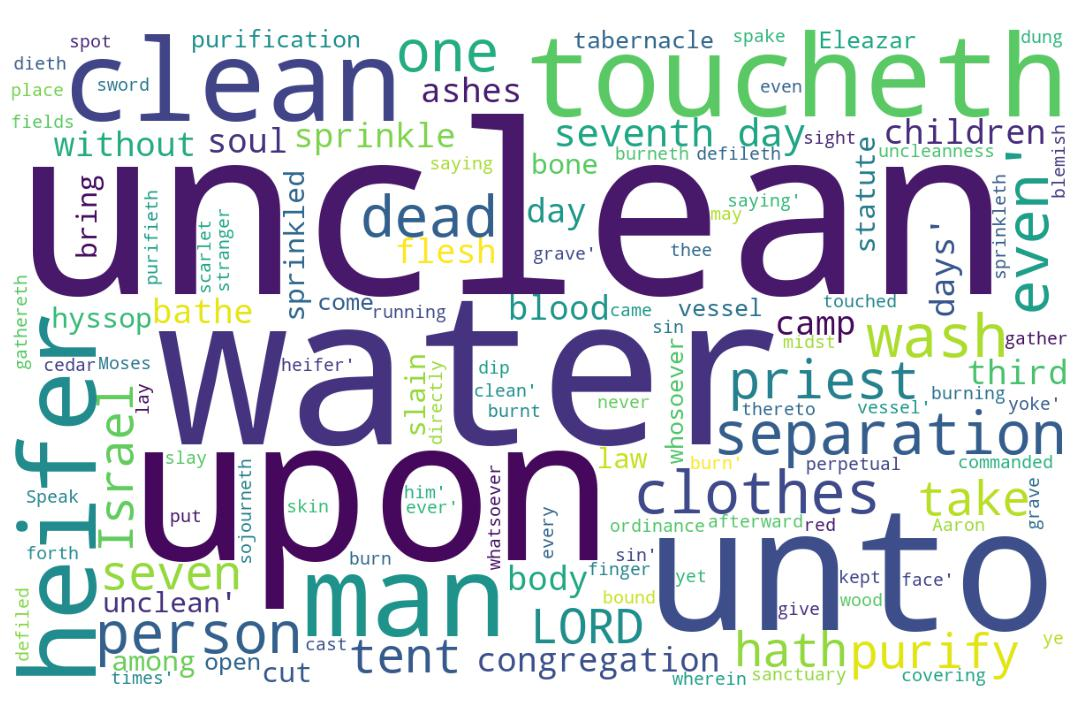
\includegraphics[width=\linewidth]{04OT-Numbers/Numbers19-WordCloud.jpg}
  \caption{Numbers 19 Word Cloud}
  \label{fig:Numbers 19 word Cloud}
\end{figure}



\marginpar{\scriptsize \centering \fcolorbox{bone}{lime}{\textbf{A RED HIEFER}}\\ (Numbers 19)
\begin{compactenum}[I.][8]
    \item  \textbf{Days} \index[scripture]{Numbers!Num 19:11} \index[scripture]{Numbers!Num 19:12} \index[scripture]{Numbers!Num 19:14}\index[scripture]{Numbers!Num 19:16}\index[scripture]{Numbers!Num 19:19} (Numbers 19:11, 12, 14, 16, 19) -- the typology of the third day and the seventh day
    \item  \textbf{Defilement} \index[scripture]{Numbers!Num 19:13} \index[scripture]{Numbers!Num 19:20} (Numbers 19:13, 20) 
    \item  \textbf{Destinations} \index[scripture]{Numbers!Num 19:03} \index[scripture]{Numbers!Num 19:07}\index[scripture]{Numbers!Num 19:09} (Numbers 19:3, 7, 9) -- inside the camp, outside the camp
    \item  \textbf{Designees}  -- the priest, the clean person, the unclean person, the dead body
    \item  \textbf{Ordinance}  \index[scripture]{Numbers!Num 19:02} (Numbers 19:2) 
    \item  \textbf{Defect} Free \index[scripture]{Numbers!Num 19:02} (Numbers 19:2) 
\end{compactenum}}

%[cmyk]{0.99998,1,0,0}{

\footnote{\textcolor[rgb]{0.00,0.25,0.00}{\hyperlink{NumbersTOC}{Return to end of Table of Contents.}}}\footnote{\href{https://audiobible.com/bible/numbers_19.html}{\textcolor[cmyk]{0.99998,1,0,0}{Numbers 19 Audio}}}\textcolor[cmyk]{0.99998,1,0,0}{And the LORD spake unto Moses and unto Aaron, saying,}
[2] \textcolor[cmyk]{0.99998,1,0,0}{This \emph{is} the ordinance of the law which the LORD hath commanded, saying, Speak unto the children of Israel, that they bring thee a red heifer without spot, wherein \emph{is} no blemish, \emph{and} upon which never came yoke:}
[3] \textcolor[cmyk]{0.99998,1,0,0}{And ye shall give her unto Eleazar the priest, that he may bring her forth without the camp, and \emph{one} shall slay her before his face:}
[4] \textcolor[cmyk]{0.99998,1,0,0}{And Eleazar the priest shall take of her blood with his finger, and sprinkle of her blood directly before the tabernacle of the congregation seven times:}
[5] \textcolor[cmyk]{0.99998,1,0,0}{And \emph{one} shall burn the heifer in his sight; her skin, and her flesh, and her blood, with her dung, shall he burn:}
[6] \textcolor[cmyk]{0.99998,1,0,0}{And the priest shall take cedar wood, and hyssop, and scarlet, and cast \emph{it} into the midst of the burning of the heifer.}
[7] \textcolor[cmyk]{0.99998,1,0,0}{Then the priest shall wash his clothes, and he shall bathe his flesh in water, and afterward he shall come into the camp, and the priest shall be unclean until the even.}
[8] \textcolor[cmyk]{0.99998,1,0,0}{And he that burneth her shall wash his clothes in water, and bathe his flesh in water, and shall be unclean until the even.}
[9] \textcolor[cmyk]{0.99998,1,0,0}{And a man \emph{that} \emph{is} clean shall gather up the ashes of the heifer, and lay \emph{them} up without the camp in a clean place, and it shall be kept for the congregation of the children of Israel for a water of separation: it \emph{is} a purification for sin.}
[10] \textcolor[cmyk]{0.99998,1,0,0}{And he that gathereth the ashes of the heifer shall wash his clothes, and be unclean until the even: and it shall be unto the children of Israel, and unto the stranger that sojourneth among them, for a statute for ever.}\\
\\
\P \textcolor[cmyk]{0.99998,1,0,0}{He that toucheth the dead body of any man shall be unclean seven days.}
[12] \textcolor[cmyk]{0.99998,1,0,0}{He shall purify himself with it on the third day, and on the seventh day he shall be clean: but if he purify not himself the third day, then the seventh day he shall not be clean.}
[13] \textcolor[cmyk]{0.99998,1,0,0}{Whosoever toucheth the dead body of any man that is dead, and purifieth not himself, defileth the tabernacle of the LORD; and that soul shall be cut off from Israel: because the water of separation was not sprinkled upon him, he shall be unclean; his uncleanness \emph{is} yet upon him.}
[14] \textcolor[cmyk]{0.99998,1,0,0}{This \emph{is} the law, when a man dieth in a tent: all that come into the tent, and all that \emph{is} in the tent, shall be unclean seven days.}
[15] \textcolor[cmyk]{0.99998,1,0,0}{And every open vessel, which hath no covering bound upon it, \emph{is} unclean.}
[16] \textcolor[cmyk]{0.99998,1,0,0}{And whosoever toucheth one that is slain with a sword in the open fields, or a dead body, or a bone of a man, or a grave, shall be unclean seven days.}
[17] \textcolor[cmyk]{0.99998,1,0,0}{And for an unclean \emph{person} they shall take of the ashes of the burnt heifer of purification for sin, and running water shall be put thereto in a vessel:}
[18] \textcolor[cmyk]{0.99998,1,0,0}{And a clean person shall take hyssop, and dip \emph{it} in the water, and sprinkle \emph{it} upon the tent, and upon all the vessels, and upon the persons that were there, and upon him that touched a bone, or one slain, or one dead, or a grave:}
[19] \textcolor[cmyk]{0.99998,1,0,0}{And the clean \emph{person} shall sprinkle upon the unclean on the third day, and on the seventh day: and on the seventh day he shall purify himself, and wash his clothes, and bathe himself in water, and shall be clean at even.}
[20] \textcolor[cmyk]{0.99998,1,0,0}{But the man that shall be unclean, and shall not purify himself, that soul shall be cut off from among the congregation, because he hath defiled the sanctuary of the LORD: the water of separation hath not been sprinkled upon him; he \emph{is} unclean.}
[21] \textcolor[cmyk]{0.99998,1,0,0}{And it shall be a perpetual statute unto them, that he that sprinkleth the water of separation shall wash his clothes; and he that toucheth the water of separation shall be unclean until even.}
[22] \textcolor[cmyk]{0.99998,1,0,0}{And whatsoever the unclean \emph{person} toucheth shall be unclean; and the soul that toucheth \emph{it} shall be unclean until even.}

\chapter{Numbers 20}

\begin{figure}
  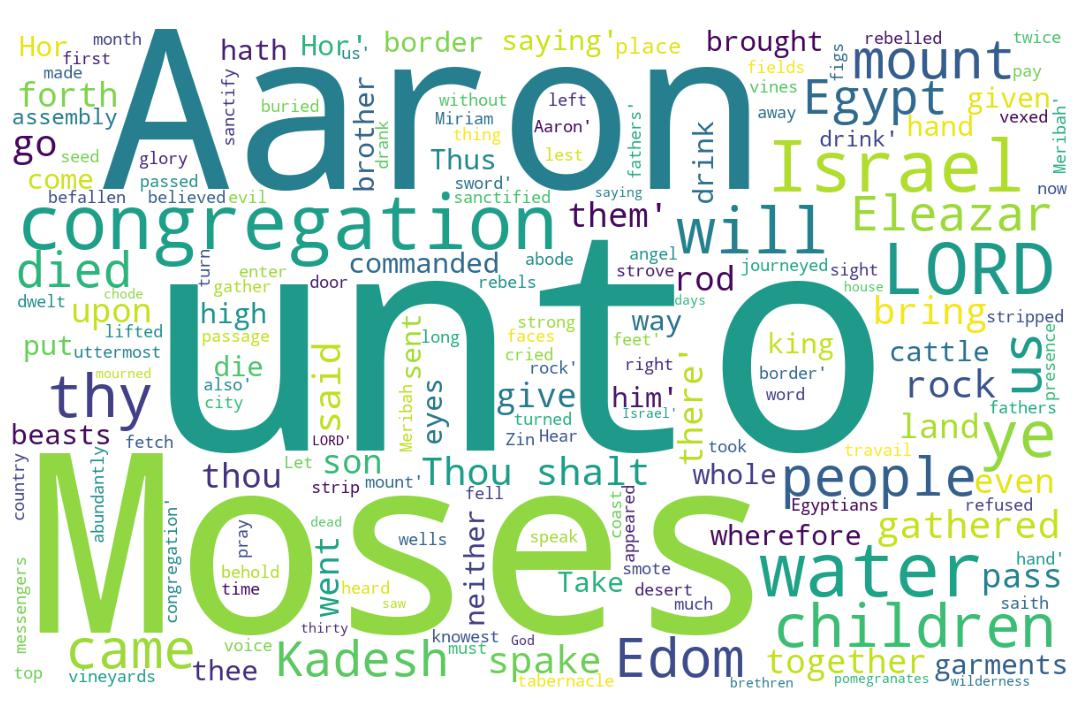
\includegraphics[width=\linewidth]{04OT-Numbers/Numbers20-WordCloud.jpg}
  \caption{Numbers 20 Word Cloud}
  \label{fig:Numbers 20 word Cloud}
\end{figure}

\marginpar{\scriptsize \centering \fcolorbox{bone}{lime}{\textbf{THE ROCK SMITTEN}}\\ (Numbers 20)
\begin{compactenum}[I.][8]
    \item  \textbf{Reaction} of Moses \index[scripture]{Numbers!Num 20:06} \index[scripture]{Numbers!Num 20:10}  (Numbers 20:6, 10)
    \item  \textbf{Rod} \index[scripture]{Numbers!Num 20:08} \index[scripture]{Numbers!Num 20:09}\index[scripture]{Numbers!Num 20:11} (Numbers 20:8, 9, 11)
    \item  \textbf{Rock} %\index[scripture]{Numbers!Num 20:11}  (Numbers 20:11) -- the typology of the third day and the seventh day
    \item  The \textbf{Rage} of Moses \index[scripture]{Numbers!Num 20:11}  (Numbers 20:11)
    \item  \textbf{Ruining} of a type \index[scripture]{Numbers!Num 20:11}  (Numbers 20:11)
    \item  \textbf{Rebels}  \index[scripture]{Numbers!Num 20:10} \index[scripture]{Numbers!Num 20:24} (Numbers 20:10, 24)
    \item  The \textbf{Revelation} -- the Law is unable to take God's people into the Promised Land %\index[scripture]{Numbers!Num 20:11}  (Numbers 20:11)
\end{compactenum}}
 
\footnote{\textcolor[rgb]{0.00,0.25,0.00}{\hyperlink{NumbersTOC}{Return to end of Table of Contents.}}}\footnote{\href{https://audiobible.com/bible/numbers_20.html}{\textcolor[cmyk]{0.99998,1,0,0}{Numbers 20 Audio}}}\textcolor[cmyk]{0.99998,1,0,0}{Then came the children of Israel, \emph{even} the whole congregation, into the desert of Zin in the first month: and the people abode in Kadesh; and Miriam died there, and was buried there.}
[2] \textcolor[cmyk]{0.99998,1,0,0}{And there was no water for the congregation: and they gathered themselves together against \fcolorbox{bone}{bone}{Moses} and against Aaron.}
[3] \textcolor[cmyk]{0.99998,1,0,0}{And the people chode with Moses, and spake, saying, Would God that we had died when our brethren died before the LORD!}
[4] \textcolor[cmyk]{0.99998,1,0,0}{And why have ye brought up the congregation of the LORD into this wilderness, that we and our cattle should die there?}
[5] \textcolor[cmyk]{0.99998,1,0,0}{And wherefore have ye made us to come up out of Egypt, to bring us in unto this evil place? it \emph{is} no place of seed, or of figs, or of vines, or of pomegranates; neither \emph{is} there any water to drink.}\
[6] \textcolor[cmyk]{0.99998,1,0,0}{And \fcolorbox{bone}{bone}{Moses} and Aaron went from the presence of the assembly unto the door of the tabernacle of the congregation, and they fell upon their faces: and the glory of the LORD appeared unto them.}\\
\\
\P \textcolor[cmyk]{0.99998,1,0,0}{And the LORD spake unto Moses, saying,}
[8] \textcolor[cmyk]{0.99998,1,0,0}{Take the rod, and gather thou the assembly together, thou, and Aaron thy brother, and speak ye unto the rock before their eyes; and it shall give forth his water, and thou shalt bring forth to them water out of the rock: so thou shalt give the congregation and their beasts drink.}
[9] \textcolor[cmyk]{0.99998,1,0,0}{And \fcolorbox{bone}{bone}{Moses} took the rod from before the LORD, as he commanded him.}
[10] \textcolor[cmyk]{0.99998,1,0,0}{And \fcolorbox{bone}{bone}{Moses} and Aaron gathered the congregation together before the rock, and he said unto them, Hear now, ye rebels; must we fetch you water out of this rock?}
[11] \textcolor[cmyk]{0.99998,1,0,0}{And \fcolorbox{bone}{bone}{Moses} lifted up his hand, and with his rod he smote the rock twice: and the water came out abundantly, and the congregation drank, and their beasts \emph{also}.}\\
\\
\P \textcolor[cmyk]{0.99998,1,0,0}{And the LORD spake unto \fcolorbox{bone}{bone}{Moses} and Aaron, Because ye believed me not, to sanctify me in the eyes of the children of Israel, therefore ye shall not bring this congregation into the land which I have given them.}
[13] \textcolor[cmyk]{0.99998,1,0,0}{This \emph{is} the water of Meribah; because the children of Israel strove with the LORD, and he was sanctified in them.}\\
\\
\P  \textcolor[cmyk]{0.99998,1,0,0}{And \fcolorbox{bone}{bone}{Moses} sent messengers from Kadesh unto the king of Edom, Thus saith thy brother Israel, Thou knowest all the travail that hath befallen us:}
[15] \textcolor[cmyk]{0.99998,1,0,0}{How our fathers went down into Egypt, and we have dwelt in Egypt a long time; and the Egyptians vexed us, and our fathers:}
[16] \textcolor[cmyk]{0.99998,1,0,0}{And when we cried unto the LORD, he heard our voice, and sent an angel, and hath brought us forth out of Egypt: and, behold, we \emph{are} in Kadesh, a city in the uttermost of thy border:}
[17] \textcolor[cmyk]{0.99998,1,0,0}{Let us pass, I pray thee, through thy country: we will not pass through the fields, or through the vineyards, neither will we drink \emph{of} the water of the wells: we will go by the king's \emph{high} way, we will not turn to the right hand nor to the left, until we have passed thy borders.}
[18] \textcolor[cmyk]{0.99998,1,0,0}{And Edom said unto him, Thou shalt not pass by me, lest I come out against thee with the sword.}
[19] \textcolor[cmyk]{0.99998,1,0,0}{And the children of Israel said unto him, We will go by the high way: and if I and my cattle drink of thy water, then I will pay for it: I will only, without \emph{doing} any thing \emph{else}, go through on my feet.}
[20] \textcolor[cmyk]{0.99998,1,0,0}{And he said, Thou shalt not go through. And Edom came out against him with much people, and with a strong hand.}
[21] \textcolor[cmyk]{0.99998,1,0,0}{Thus Edom refused to give Israel passage through his border: wherefore Israel turned away from him.}\\
\\
\P \textcolor[cmyk]{0.99998,1,0,0}{And the children of Israel, \emph{even} the whole congregation, journeyed from Kadesh, and came unto mount Hor.}
[23] \textcolor[cmyk]{0.99998,1,0,0}{And the LORD spake unto \fcolorbox{bone}{bone}{Moses} and Aaron in mount Hor, by the coast of the land of Edom, saying,}
[24] \textcolor[cmyk]{0.99998,1,0,0}{Aaron shall be gathered unto his people: for he shall not enter into the land which I have given unto the children of Israel, because ye rebelled against my word at the water of Meribah.}
[25] \textcolor[cmyk]{0.99998,1,0,0}{Take Aaron and Eleazar his son, and bring them up unto mount Hor:}
[26] \textcolor[cmyk]{0.99998,1,0,0}{And strip Aaron of his garments, and put them upon Eleazar his son: and Aaron shall be gathered \emph{unto} \emph{his} \emph{people}, and shall die there.}
[27] \textcolor[cmyk]{0.99998,1,0,0}{And \fcolorbox{bone}{bone}{Moses} did as the LORD commanded: and they went up into mount Hor in the sight of all the congregation.}
[28] \textcolor[cmyk]{0.99998,1,0,0}{And \fcolorbox{bone}{bone}{Moses} stripped Aaron of his garments, and put them upon Eleazar his son; and Aaron died there in the top of the mount: and \fcolorbox{bone}{bone}{Moses} and Eleazar came down from the mount.}
[29] \textcolor[cmyk]{0.99998,1,0,0}{And when all the congregation saw that Aaron was dead, they mourned for Aaron thirty days, \emph{even} all the house of Israel.}
\chapter{Numbers 21}


\begin{figure}
  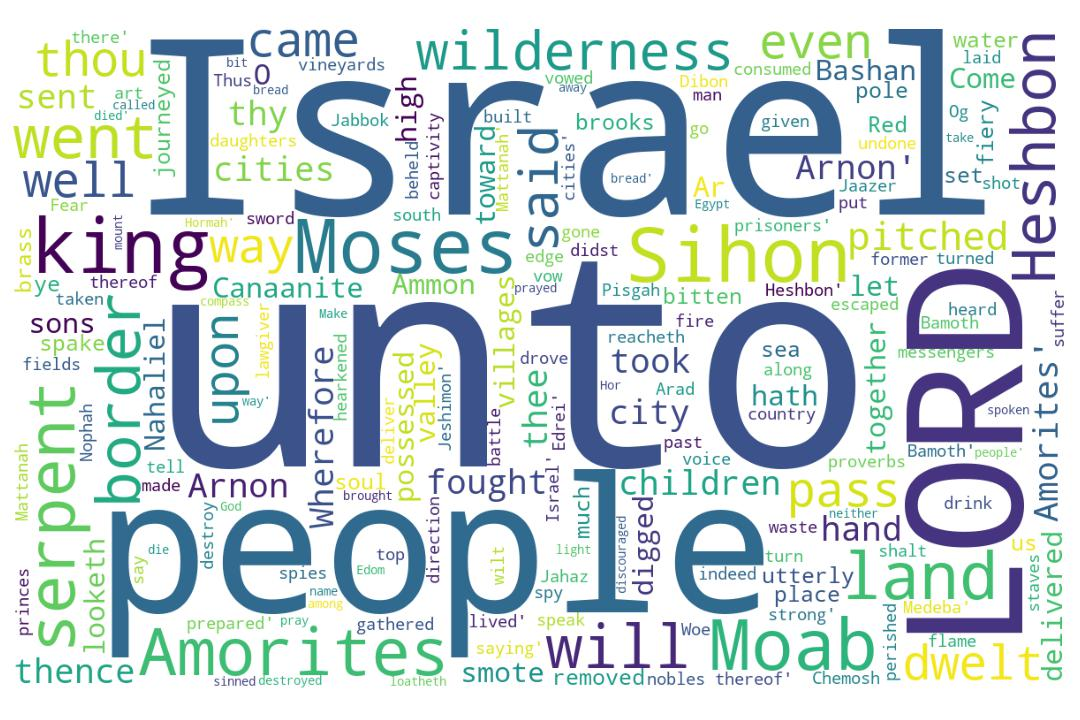
\includegraphics[width=\linewidth]{04OT-Numbers/Numbers21-WordCloud.jpg}
  \caption{Numbers 21 Word Cloud}
  \label{fig:Numbers 21 word Cloud}
\end{figure}


\marginpar{\scriptsize \centering \fcolorbox{bone}{lime}{\textbf{SIN, SERPENTS \& SWORDS}}\\ (Numbers 21)
\begin{compactenum}[I.][8]
     \item  The \textbf{Sin} of Discouragement \index[scripture]{Numbers!Num 21:04}   (Numbers 21:4)
    \item  \textbf{Serpents}  \index[scripture]{Numbers!Num 21:06}   (Numbers 21:6)
    \item  \textbf{Supplication}  \index[scripture]{Numbers!Num 21:07}   (Numbers 21:7)
    \item  The \textbf{Symbol}  \index[scripture]{Numbers!Num 21:09}   (Numbers 21:9)
    \item  A \textbf{Song}  \index[scripture]{Numbers!Num 21:17}   (Numbers 21:17)
    \item  The \textbf{Sword}  \index[scripture]{Numbers!Num 21:24}   (Numbers 21:24)
\end{compactenum}}




\footnote{\textcolor[rgb]{0.00,0.25,0.00}{\hyperlink{NumbersTOC}{Return to end of Table of Contents.}}}\footnote{\href{https://audiobible.com/bible/numbers_21.html}{\textcolor[cmyk]{0.99998,1,0,0}{Numbers 21 Audio}}}\textcolor[cmyk]{0.99998,1,0,0}{And \emph{when} king Arad the Canaanite, which dwelt in the south, heard tell that Israel came by the way of the spies; then he fought against Israel, and took \emph{some} of them prisoners.}
[2] \textcolor[cmyk]{0.99998,1,0,0}{And Israel vowed a vow unto the LORD, and said, If thou wilt indeed deliver this people into my hand, then I will utterly destroy their cities.}
[3] \textcolor[cmyk]{0.99998,1,0,0}{And the LORD hearkened to the voice of Israel, and delivered up the Canaanites; and they utterly destroyed them and their cities: and he called the name of the place Hormah.}\\
\\
\P \textcolor[cmyk]{0.99998,1,0,0}{And they journeyed from mount Hor by the way of the Red sea, to compass the land of Edom: and the soul of the people was much discouraged because of the way.}
[5] \textcolor[cmyk]{0.99998,1,0,0}{And the people spake against God, and against Moses, Wherefore have ye brought us up out of Egypt to die in the wilderness? for \emph{there} \emph{is} no bread, neither \emph{is} \emph{there} \emph{any} water; and our soul loatheth this light bread.}
[6] \textcolor[cmyk]{0.99998,1,0,0}{And the LORD sent fiery serpents among the people, and they bit the people; and much people of Israel died.}\\
\\
\P \textcolor[cmyk]{0.99998,1,0,0}{Therefore the people came to Moses, and said, We have sinned, for we have spoken against the LORD, and against thee; pray unto the LORD, that he take away the serpents from us. And Moses prayed for the people.}
[8] \textcolor[cmyk]{0.99998,1,0,0}{And the LORD said unto Moses, Make thee a fiery serpent, and set it upon a pole: and it shall come to pass, that every one that is bitten, when he looketh upon it, shall live.}
[9] \textcolor[cmyk]{0.99998,1,0,0}{And Moses made a serpent of brass, and put it upon a pole, and it came to pass, that if a serpent had bitten any man, when he beheld the serpent of brass, he lived.}\\
\\
\P \textcolor[cmyk]{0.99998,1,0,0}{And the children of Israel set forward, and pitched in Oboth.}
[11] \textcolor[cmyk]{0.99998,1,0,0}{And they journeyed from Oboth, and pitched at Ije-abarim, in the wilderness which \emph{is} before Moab, toward the sunrising.}
[12] \textcolor[cmyk]{0.99998,1,0,0}{From thence they removed, and pitched in the valley of Zared.}
[13] \textcolor[cmyk]{0.99998,1,0,0}{From thence they removed, and pitched on the other side of Arnon, which \emph{is} in the wilderness that cometh out of the coasts of the Amorites: for Arnon \emph{is} the border of Moab, between Moab and the Amorites.}
[14] \textcolor[cmyk]{0.99998,1,0,0}{Wherefore it is said in the book of the wars of the LORD, What he did in the Red sea, and in the brooks of Arnon,}
[15] \textcolor[cmyk]{0.99998,1,0,0}{And at the stream of the brooks that goeth down to the dwelling of Ar, and lieth upon the border of Moab.}
[16] \textcolor[cmyk]{0.99998,1,0,0}{And from thence \emph{they} \emph{went} to Beer: that \emph{is} the well whereof the LORD spake unto Moses, Gather the people together, and I will give them water.}
[17] \textcolor[cmyk]{0.99998,1,0,0}{Then Israel sang this song, Spring up, O well; sing ye unto it:}
[18] \textcolor[cmyk]{0.99998,1,0,0}{The princes digged the well, the nobles of the people digged it, by \emph{the} \emph{direction} \emph{of} the lawgiver, with their staves. And from the wilderness \emph{they} \emph{went} to Mattanah:}
[19] \textcolor[cmyk]{0.99998,1,0,0}{And from Mattanah to Nahaliel: and from Nahaliel to Bamoth:}
[20] \textcolor[cmyk]{0.99998,1,0,0}{And from Bamoth \emph{in} the valley, that \emph{is} in the country of Moab, to the top of Pisgah, which looketh toward Jeshimon.}\\
\\
\P \textcolor[cmyk]{0.99998,1,0,0}{And Israel sent messengers unto Sihon king of the Amorites, saying,}
[22] \textcolor[cmyk]{0.99998,1,0,0}{Let me pass through thy land: we will not turn into the fields, or into the vineyards; we will not drink \emph{of} the waters of the well: \emph{but} we will go along by the king's \emph{high} way, until we be past thy borders.}
[23] \textcolor[cmyk]{0.99998,1,0,0}{And Sihon would not suffer Israel to pass through \fcolorbox{bone}{bone}{his} border: but Sihon gathered all \fcolorbox{bone}{bone}{his} people together, and went out against Israel into the wilderness: and he came to Jahaz, and fought against Israel.}
[24] \textcolor[cmyk]{0.99998,1,0,0}{And Israel smote him with the edge of the sword, and possessed \fcolorbox{bone}{bone}{his} land from Arnon unto Jabbok, even unto the children of Ammon: for the border of the children of Ammon \emph{was} strong.}
[25] \textcolor[cmyk]{0.99998,1,0,0}{And Israel took all these cities: and Israel dwelt in all the cities of the Amorites, in Heshbon, and in all the villages thereof.}
[26] \textcolor[cmyk]{0.99998,1,0,0}{For Heshbon \emph{was} the city of Sihon the king of the Amorites, who had fought against the former king of Moab, and taken all \fcolorbox{bone}{bone}{his} land out of \fcolorbox{bone}{bone}{his} hand, even unto Arnon.}
[27] \textcolor[cmyk]{0.99998,1,0,0}{Wherefore they that speak in proverbs say, Come into Heshbon, let the city of Sihon be built and prepared:}
[28] \textcolor[cmyk]{0.99998,1,0,0}{For there is a fire gone out of Heshbon, a flame from the city of Sihon: it hath consumed Ar of Moab, \emph{and} the lords of the high places of Arnon.}
[29] \textcolor[cmyk]{0.99998,1,0,0}{Woe to thee, Moab! thou art undone, O people of Chemosh: he hath given \fcolorbox{bone}{bone}{his} sons that escaped, and \fcolorbox{bone}{bone}{his} daughters, into captivity unto Sihon king of the Amorites.}
[30] \textcolor[cmyk]{0.99998,1,0,0}{We have shot at them; Heshbon is perished even unto Dibon, and we have laid them waste even unto Nophah, which \emph{reacheth} unto Medeba.}\\
\\
\P \textcolor[cmyk]{0.99998,1,0,0}{Thus Israel dwelt in the land of the Amorites.}
[32] \textcolor[cmyk]{0.99998,1,0,0}{And Moses sent to spy out Jaazer, and they took the villages thereof, and drove out the Amorites that \emph{were} there.}
[33] \textcolor[cmyk]{0.99998,1,0,0}{And they turned and went up by the way of Bashan: and Og the king of Bashan went out against them, he, and all \fcolorbox{bone}{bone}{his} people, to the battle at Edrei.}
[34] \textcolor[cmyk]{0.99998,1,0,0}{And the LORD said unto Moses, Fear him not: for I have delivered him into thy hand, and all \fcolorbox{bone}{bone}{his} people, and \fcolorbox{bone}{bone}{his} land; and thou shalt do to him as thou didst unto Sihon king of the Amorites, which dwelt at Heshbon.}
[35] \textcolor[cmyk]{0.99998,1,0,0}{So they smote him, and \fcolorbox{bone}{bone}{his} sons, and all \fcolorbox{bone}{bone}{his} people, until there was none left him alive: and they possessed \fcolorbox{bone}{bone}{his} land.}

\chapter{Psalm 47}

\begin{figure}
  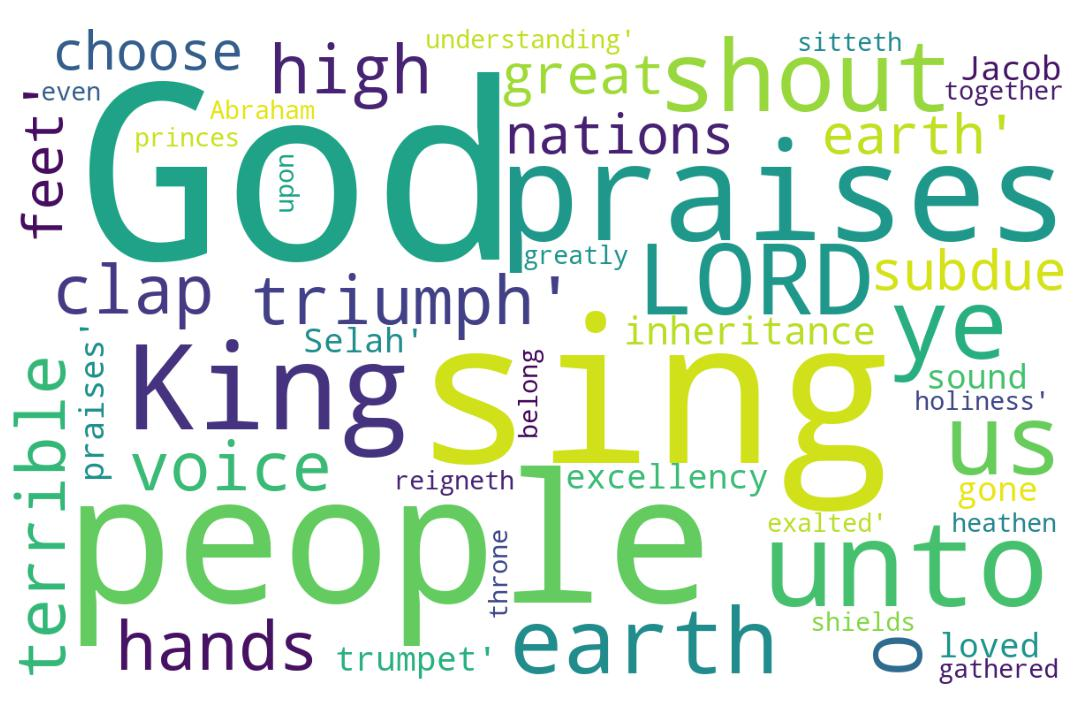
\includegraphics[width=\linewidth]{19OT-Psalms/Psalm47-WordCloud.jpg}
  \caption{Psalm 47 Word Cloud}
  \label{fig:Psalm 47 word Cloud}
\end{figure}

\marginpar{\scriptsize \centering \fcolorbox{bone}{lime}{\textbf{THE REIGNING KING}}\\ (Psalm 47:1-9) \begin{compactenum}[I.][8]
    \item The \textbf{Chronology} of end-time Events \index[scripture]{Psalms!Psa 044}\index[scripture]{Psalms!Psa 045}\index[scripture]{Psalms!Psa 046}\index[scripture]{Psalms!Psa 047} (Psa 44-47)
    \item The \textbf{Culmination} of History \index[scripture]{Psalms!Psa 047:02} (Psa 47:2)
    \item The \textbf{Command} of this King \index[scripture]{Psalms!Psa 047:02} (Psa 47:2)
    \item The \textbf{Conquests} of this King \index[scripture]{Psalms!Psa 047:03} (Psa 47:3)
    \item The \textbf{Concern} of this King \index[scripture]{Psalms!Psa 047:04} (Psa 47:4)
    \item The \textbf{Chorus} of Praise \index[scripture]{Psalms!Psa 047:06} (Psa 47:6)
    \item The \textbf{King} enthroned \index[scripture]{Psalms!Psa 047:07} (Psa 47:7)
\end{compactenum}}
    
%%%%%%%%%%%%%%%%%%%%%%%%%%%%%%
%%%%%%%%%%%%%%%%%%%%%%%%%%%%%%
\footnote{\textcolor[cmyk]{0.99998,1,0,0}{\hyperlink{TOC}{Return to end of Table of Contents.}}}\footnote{\href{https://audiobible.com/bible/psalms_47.html}{\textcolor[cmyk]{0.99998,1,0,0}{Psalms Audio}}}\textcolor[cmyk]{0.99998,1,0,0}{To the chief Musician, A Psalm for the sons of Korah.}\\
\\
\textcolor[cmyk]{0.99998,1,0,0}{O clap your hands, all ye people; shout unto God with the voice of triumph.}
[2] \textcolor[cmyk]{0.99998,1,0,0}{For the LORD most high \emph{is} terrible; \emph{he} \emph{is} a great King over all the earth.}\footnote{\textbf{Zechariah 14:9}  - And the LORD shall be king over all the earth: in that day shall there be one LORD, and his name one.}
[3] \textcolor[cmyk]{0.99998,1,0,0}{He shall subdue the people under us, and the nations under our feet.}\footnote{\textbf{Philippians 3:21} - Who shall change our vile body, that it may be fashioned like unto his glorious body, according to the working whereby he is able even to subdue all things unto himself.}
[4] \textcolor[cmyk]{0.99998,1,0,0}{He shall choose our inheritance for us, the excellency of Jacob whom he loved. Selah.}
[5] \textcolor[cmyk]{0.99998,1,0,0}{God is gone up with a shout, the LORD with the sound of a trumpet.}
[6] \textcolor[cmyk]{0.99998,1,0,0}{Sing praises to God, sing praises: sing praises unto our King, sing praises.}
[7] \textcolor[cmyk]{0.99998,1,0,0}{For God \emph{is} the King of all the earth: sing ye praises with \fcolorbox{bone}{MYGOLD}{understanding}.}
[8] \textcolor[cmyk]{0.99998,1,0,0}{God reigneth over the heathen: God sitteth upon the throne of his holiness.}
[9] \textcolor[cmyk]{0.99998,1,0,0}{The princes of the people are gathered together, \emph{even} the people of the God of Abraham: for the shields of the earth \emph{belong} unto God: he is greatly exalted.}\footnote{\textbf{Genesis 26:24} - And the LORD appeared unto him the same night, and said, I am the God of Abraham thy father: fear not, for I am with thee, and will bless thee, and multiply thy seed for my servant Abraham’s sake.}\footnote{\textbf{Exodus 3:6} - Moreover he said, I am the God of thy father, the God of Abraham, the God of Isaac, and the God of Jacob. And Moses hid his face; for he was afraid to look upon God.}\footnote{\textbf{Acts 7:32} - Saying, I am the God of thy fathers, the God of Abraham, and the God of Isaac, and the God of Jacob. Then Moses trembled, and durst not behold.}

 \chapter{Proverb 16}
 
\begin{figure}
  \includegraphics[width=\linewidth]{20OT-Proverbs/Proverb16-Wordcloud.jpg}
  \caption{Proverb 16 Word Cloud}
  \label{fig:Proverb 16 word Cloud}
\end{figure}

\marginpar{\scriptsize \centering \fcolorbox{bone}{lime}{\textbf{PRAYERS FOR THE FAITHFUL}}\\ (Proverb 16:1-33) \begin{compactenum}[I.][8]
    \item \textbf{Prepare my Heart}  \index[scripture]{Proverbs!Pro 16:01}(Pro 16:1)
    \item \textbf{Peruse my Ways} \index[scripture]{Proverbs!Pro 16:02}(Pro 16:2)
    \item \textbf{Purify my Thoughts} \index[scripture]{Proverbs!Pro 16:03}(Pro 16:3)
    \item \textbf{Point out the Path} \index[scripture]{Proverbs!Pro 16:09}(Pro 16:9)
    \item \textbf{Passify my Anger} \index[scripture]{Proverbs!Pro 16:14}(Pro 16:14)
    \item \textbf{Preserve my Soul} \index[scripture]{Proverbs!Pro 16:17}(Pro 16:17)
    \item \textbf{Impart Wisdom} \index[scripture]{Proverbs!Pro 16:21}(Pro 16:21)
\end{compactenum}}

\marginpar{\scriptsize \centering \fcolorbox{bone}{yellow}{\textbf{A GODLY MAN}}\\ (Proverb 16:1-33) \begin{compactenum}[I.][8]
    \item Is \textbf{Prepared}  \index[scripture]{Proverbs!Pro 16:01} (Pro 16:1)
    \item Is \textbf{Purposed}  \index[scripture]{Proverbs!Pro 16:03} (Pro 16:3)
    \item Has \textbf{Purged} Iniquity  \index[scripture]{Proverbs!Pro 16:06} (Pro 16:6)
    \item Is \textbf{Peaceable}   \index[scripture]{Proverbs!Pro 16:07} (Pro 16:7)
    \item Is \textbf{Preserved}   \index[scripture]{Proverbs!Pro 16:17} (Pro 16:17)
    \item Is not \textbf{Proud}   \index[scripture]{Proverbs!Pro 16:19} (Pro 16:19)
    \item Is \textbf{Prudent}   \index[scripture]{Proverbs!Pro 16:21} (Pro 16:21)
\end{compactenum}}

\marginpar{\scriptsize \centering \fcolorbox{bone}{black}{\textbf{\textcolor[cmyk]{0,0,0,0}{GOD IN CONTROL}}}\\ (Proverb 16) 
 \begin{compactenum}[I.][8]
	\item \textbf{Determined Spirits} \index[scripture]{Proverbs!Pro 16:09} (Pro 16:9)
	\item \textbf{Directed Steps}  \index[scripture]{Proverbs!Pro 16:09} (Pro 16:9)
	\item A \textbf{Divine Sentence}  \index[scripture]{Proverbs!Pro 16:10}  (Pro 16:10)
	\item \textbf{Destroyed Soul}  \index[scripture]{Proverbs!Pro 16:18}  (Pro 16:18)
	\item A \textbf{Delighted Soul}  \index[scripture]{Proverbs!Pro 16:19}  (Pro 16:19)
	\item \textbf{Dug-up Sorrows}  \index[scripture]{Proverbs!Pro 16:27} (Pro 16:27)
	\item A \textbf{Disciplined Spirit}  \index[scripture]{Proverbs!Pro 16:32} (Pro 16:32)
\end{compactenum}}

\footnote{\textcolor[cmyk]{0.99998,1,0,0}{\hyperlink{TOC}{Return to end of Table of Contents.}}}\footnote{\href{https://audiobible.com/bible/proverbs_16.html}{\textcolor[cmyk]{0.99998,1,0,0}{Proverbs Audio}}}\textcolor[cmyk]{0.99998,1,0,0}{The \fcolorbox{bone}{lime}{preparations of the heart} in man, and the answer of the tongue, \emph{is} from the LORD.}
[2] \textcolor[cmyk]{0.99998,1,0,0}{All the ways of a man \emph{are} clean in his own eyes; but the \fcolorbox{bone}{lime}{LORD} \fcolorbox{bone}{lime}{weigheth} \fcolorbox{bone}{lime}{the} \fcolorbox{bone}{lime}{spirits}.}
[3] \textcolor[cmyk]{0.99998,1,0,0}{Commit thy works unto the LORD, and thy \fcolorbox{bone}{lime}{thoughts shall be} \fcolorbox{bone}{lime}{established}.}
[4] \textcolor[cmyk]{0.99998,1,0,0}{The LORD hath made all \emph{things} for himself: yea, even the wicked for the day of evil.}
[5] \textcolor[cmyk]{0.99998,1,0,0}{Every one \emph{that} \emph{is} proud in heart \emph{is} an abomination to the LORD: \emph{though} hand \emph{join} in hand, he shall not be unpunished.}
[6] \textcolor[cmyk]{0.99998,1,0,0}{By mercy and truth iniquity is purged: and by the fear of the LORD \emph{men} depart from evil.}
[7] \textcolor[cmyk]{0.99998,1,0,0}{When a man's ways please the LORD, he maketh even his enemies to be at peace with him.}
[8] \textcolor[cmyk]{0.99998,1,0,0}{Better \emph{is} a little with \fcolorbox{bone}{MYGOLD}{righteousness} than great revenues without right.}
[9] \textcolor[cmyk]{0.99998,1,0,0}{A man's heart deviseth his way: but the \fcolorbox{bone}{lime}{LORD directeth his steps}.}
[10] \textcolor[cmyk]{0.99998,1,0,0}{A divine sentence \emph{is} in the lips of the king: his mouth \fcolorbox{bone}{MYGOLD}{transgresseth} not in judgment.}
[11] \textcolor[cmyk]{0.99998,1,0,0}{A just weight and balance \emph{are} the LORD'S: all the weights of the bag \emph{are} his work.}
[12] \textcolor[cmyk]{0.99998,1,0,0}{\emph{It} \emph{is} an abomination to kings to commit wickedness: for the throne is established by \fcolorbox{bone}{MYGOLD}{righteousness}.}
[13] \textcolor[cmyk]{0.99998,1,0,0}{Righteous lips \emph{are} the delight of kings; and they love him that speaketh right.}
[14] \textcolor[cmyk]{0.99998,1,0,0}{The wrath of a king \emph{is} \emph{as} messengers of death: but a \fcolorbox{bone}{lime}{wise man will pacify it}.}
[15] \textcolor[cmyk]{0.99998,1,0,0}{In the light of the king's countenance \emph{is} life; and his favour \emph{is} as a cloud of the latter rain.}
[16] \textcolor[cmyk]{0.99998,1,0,0}{How much better \emph{is} \emph{it} to get wisdom than gold! and to get \fcolorbox{bone}{MYGOLD}{understanding} rather to be chosen than silver!}
[17] \textcolor[cmyk]{0.99998,1,0,0}{The highway of the upright \emph{is} to depart from evil: he that keepeth his way \fcolorbox{bone}{lime}{preserveth} his soul.}
[18] \textcolor[cmyk]{0.99998,1,0,0}{Pride \emph{goeth} before destruction, and an haughty spirit before a fall.}
[19] \textcolor[cmyk]{0.99998,1,0,0}{Better \emph{it} \emph{is} \emph{to} \emph{be} of an humble spirit with the lowly, than to divide the spoil with the proud.}
[20] \textcolor[cmyk]{0.99998,1,0,0}{He that handleth a matter wisely shall find good: and whoso trusteth in the LORD, happy \emph{is} he.}
[21] \textcolor[cmyk]{0.99998,1,0,0}{The \fcolorbox{bone}{lime}{wise in heart} shall be called prudent: and the sweetness of the lips increaseth learning.}
[22] \textcolor[cmyk]{0.99998,1,0,0}{\fcolorbox{bone}{MYGOLD}{Understanding} \emph{is} a wellspring of life unto him that hath it: but the instruction of fools \emph{is} folly.}\footnote{\textbf{Proverbs 18:4} - The words of a man’s mouth are as deep waters, and the wellspring of wisdom as a flowing brook.}\marginpar{ \scriptsize  {\textcolor[rgb]{0.00,0.545,0.269}{$\rightarrow$``wellspring'' found ONLY here and in Proverbs 18:4.}}}
[23] \textcolor[cmyk]{0.99998,1,0,0}{The heart of the wise teacheth his mouth, and addeth learning to his lips.}
[24] \textcolor[cmyk]{0.99998,1,0,0}{Pleasant words \emph{are} \emph{as} an honeycomb, sweet to the soul, and health to the bones.}
[25] \textcolor[cmyk]{0.99998,1,0,0}{There is a way that seemeth right unto a man, but the end thereof \emph{are} the ways of death.}
[26] \textcolor[cmyk]{0.99998,1,0,0}{He that laboureth laboureth for himself; for his mouth craveth it of him.}
[27] \textcolor[cmyk]{0.99998,1,0,0}{An ungodly man diggeth up evil: and in his lips \emph{there} \emph{is} as a burning fire.}
[28] \textcolor[cmyk]{0.99998,1,0,0}{A froward man soweth strife: and a whisperer separateth chief friends.}\footnote{\textbf{Proverb 6:14} - Frowardness is in his heart, he deviseth mischief continually; he soweth discord.}\footnote{\textbf{Proverb 6:19} - A false witness that speaketh lies, and he that soweth discord among brethren.}
[29] \textcolor[cmyk]{0.99998,1,0,0}{A violent man enticeth his neighbour, and leadeth him into the way \emph{that} \emph{is} not good.}
[30] \textcolor[cmyk]{0.99998,1,0,0}{He shutteth his eyes to devise froward things: moving his lips he bringeth evil to pass.}
[31] \textcolor[cmyk]{0.99998,1,0,0}{The hoary head \emph{is} a crown of glory, \emph{if} it be found in the way of \fcolorbox{bone}{MYGOLD}{righteousness}.}
[32] \textcolor[cmyk]{0.99998,1,0,0}{\emph{He} \emph{that} \emph{is} slow to anger \emph{is} better than the mighty; and he that ruleth his spirit than he that taketh a city.}
[33] \textcolor[cmyk]{0.99998,1,0,0}{The lot is cast into the lap; but the whole disposing thereof \emph{is} of the LORD.}




\end{document}

